
\chapter{Data Cleaning}
\label{DataCleaning}

The TC1a is a large complex data set with a lot of missing values, close to 50\% in the evening peak period that is to be analysed. In order to find enough coherent data to perform analysis a significant amount of data wrangling is required. The following chapter describes the method used for cleaning the data and shows the results of the cleaning process. It also gives a brief look at the statistical qualities of the data. An overview of the data cleaning process can be seen as a flowchart in Figure \ref{fig:CleanFlow}.
As mentioned in chapter \ref{DataDesc}, the data set is comprised of 8798 smart meters and covers 883 days from 01-05-2011 to 30-09-2013, data is made up of 30 minute time periods.

\begin{figure}[ht]
    \centering
    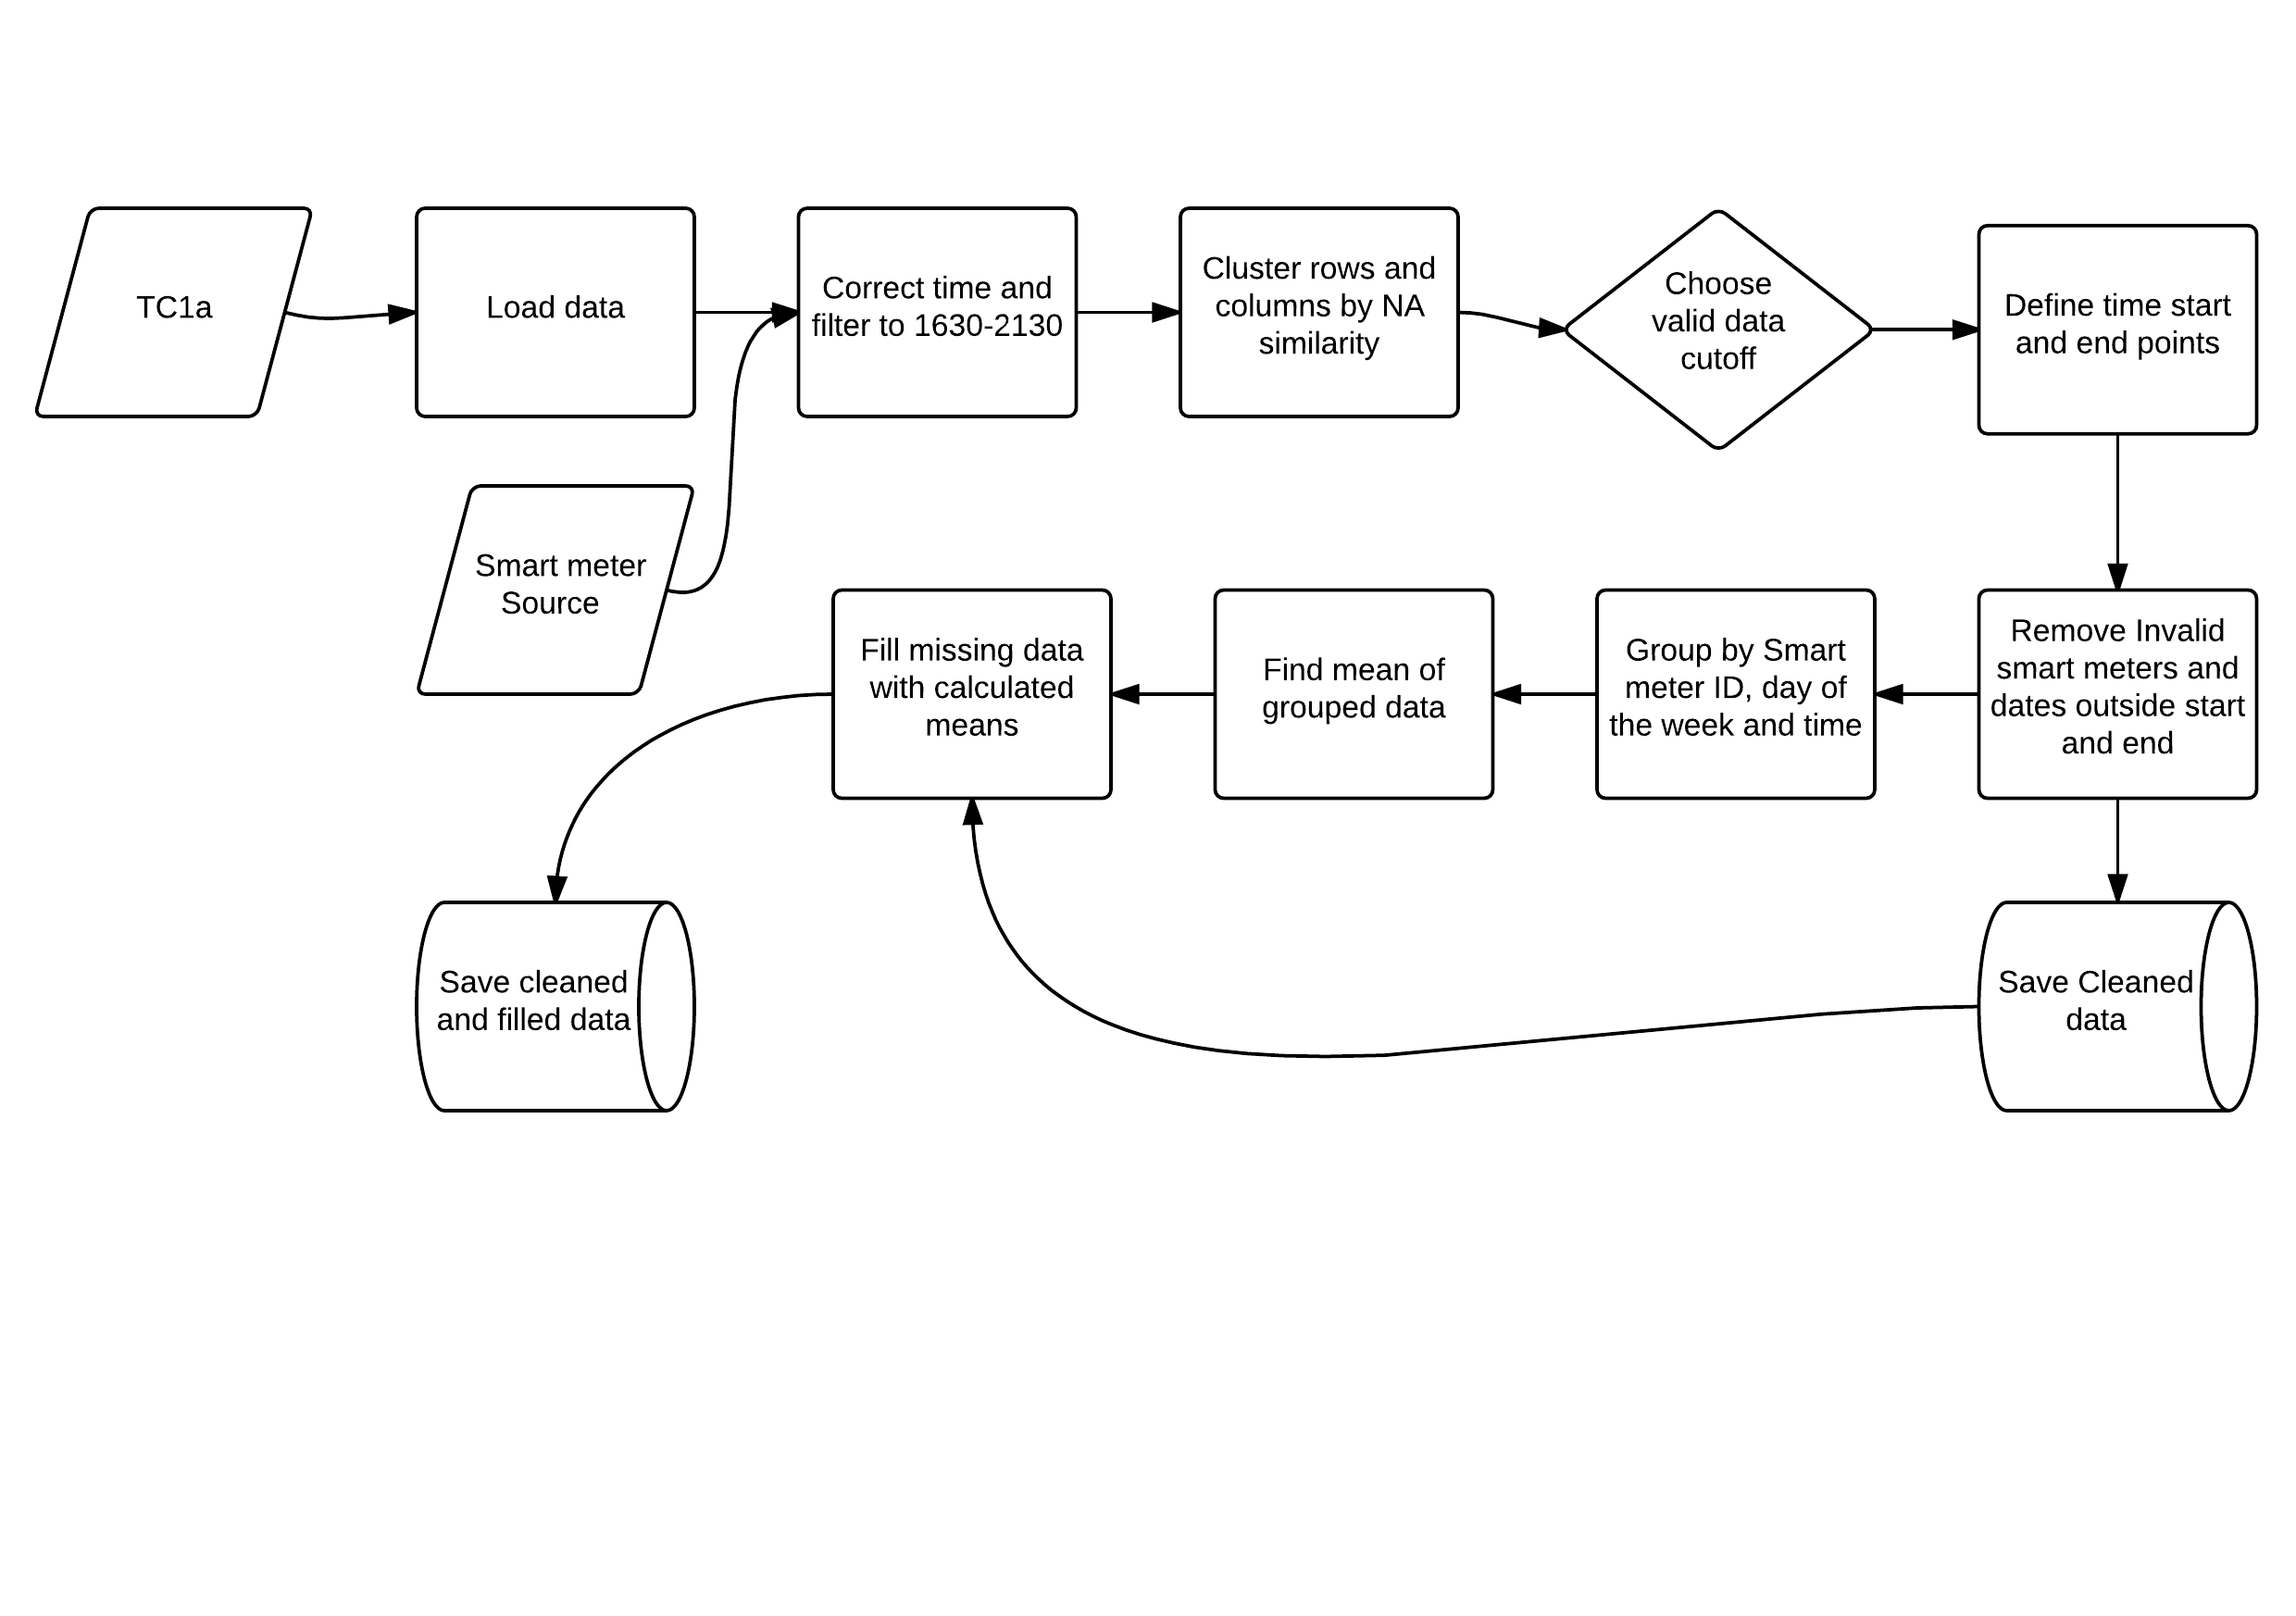
\includegraphics[width =\textwidth]{Figures/Appendix/DataCleaning.png}
    \caption[Data cleaning process]{Flow chart of the Data Cleaning Process}
    \label{fig:CleanFlow}
\end{figure}


\section{Method}

After loading the dataset, the timestamps need to be adjusted in order to take account of the different timezones used by the smart meters as mentioned in Chapter \ref{DataDesc}, so that when time filtering occurs, the correct time periods are taken for all smart meters and that usage is consistent across both smart meter brands. The time zone used will be local time, which is "Europe/London" from the the IANA timezone database \cite{iananumberresources1918}.

Once the timestamps have been adjusted the time periods will be filtered to the hours under investigation i.e 1600-2130. These hours have been chosen as this time period is of key interest to suppliers as consumption peaks when consumers return home in the evening, as a result the absolute value and variability is higher than other times during the day. This will reduce the amount of cleaning required to only that which will eventually be used and prevent confusing the cleaning process with irrelevant information. 

Once filtered the data is changed from long format to wide format in accordance with tidy data principles \cite{wickham2014}. This results in a data frame or matrix that is 8799 columns wide, with each column representing a smart meter plus the datetime column, and 1065 rows, where each row represents a half hour time period. The spreading process makes all smart meters present across all periods. Where smart meters did not send a time stamped data point either because they weren't installed or there was a transmission error, the data is classed as missing and filled with NA values.

In order to make sure the data is clean enough to be used, the data will be checked for missingness. Depending on the nature of the missingness different actions will be taken, low levels of missingness can either be removed, filled using an average, or filled using multiple imputation \cite{lee2013}. Due to the size of the dataset multiple imputation will not be considered as the resulting dataset will require a large amount of computation without having a clear payoff, however this approach can change once more information about the dataset is known. 

If the data is MNAR (Missing Not At Random) then the structure of the missingness will need to be analysed in order to find meter/day combinations that provide high levels of non-missingness, the remaining data will then be excluded from the rest of the process. The structure of the missingness will be visualised using an aggregated heatmap with both the time and smart meter axis ordered by hierarchical similarity. This method which was developed for this project takes a logical matrix where 1 represents valid data and 0 represents NA. The rows and columns of the matrix then make up individual vectors. The vectors of each row can be compared to each other using hierarchical clustering specifically the agglomerative Lance-Williams recursive clustering algorithm \cite{lance1967}. This clustering repeatedly groups the vectors by similarity, using the correlation matrix of the vectors, until all vectors have been grouped into a single cluster that represents the entire dataset. The order that the vectors were merged in created a new vector which is can be used to rearrange the vectors by hierarchical similarity, if both the time and smart meter dimensions of the data are rearranged the structural missingness of the data will be revealed see Figure \ref{fig:unordered} compared to Figure \ref{fig:ordered}. However with large datasets there can be so many vectors that the resulting organised matrix when visualised is difficult to interpret or computationally challenging to visualise. In order to resolve this, the orderd matrix is aggregated along the x and y axis by an appropriate amount, in the case of this data set the smart meters and time periods were aggregated by 5 each reducing the matrix by 25. This aggregation technique produces a value between 0 and 1 for an NA logical matrix. This technique is only appropriate after ordering by hierarchical similarity as it minimises the information loss caused by the aggregation process. The heatmap visualisation process will be used throughout the project in order to visualise similarity.

Using the heatmap the most valuable smart meters will be identified and isolated using a balance of least NA's and part of a large block of smart meters with a similar NA pattern. the next step will plot the minimum percentage of valid (non-missing) data required for each half-hour time period to be included in the dataset. After considering the volume/quality trade off on time periods, a cut off point will be chosen and all time periods which do not meet the minimum cut off criteria will be removed, and the same process repeated using smart meters. the resulting dataset will be a high quality subset of the original dataset, with relatively few missing values.

\subsection{Imputing missing values}
\label{sec:imputation}
As a large amount of the project involves the creation of similarity matrices, any NA values have the potential to invalidate the similarity score between any given smart meter pair. To prevent this the remaining NA's will be filled using the the half hour mean for that weekday for that smart meter for all values that are not NA. This runs the risk of some NA's being filled with unrealistic data, however the total number of NA's is likely to be so low that it doesn't have a significant effect on the overall result. In order to ensure that the data was as full as possible individual days that did not make the cut of minimum number of valid cells are re-included and the missing values included in the imputation process.

\section{Results}

Initial visual analysis of missingness was not very revealing as shown in figure \ref{fig:unordered}. In order to uncover any structure in the missingness, the rows and columns were ordered by the hierarchical similarity of the respective axis, this means that time periods that are most similar in their missingness are arranged together and smart meters that are most similar in their missingness are also arranged together. The resulting ordered missingness map is shown in figure \ref{fig:ordered}. It revealed that there was a high amount of missing data and that the data was Missing Not At Random (MNAR). In total 48\% of the dataset was missing values, according to the CLNR the majority of these losses were due to customer action \cite{howard2015}. To find which smart meters to extract, the amount of non missing data was plotted in the same order as the clustered smart meters, the results are shown in figure \ref{fig:breakpoints}. The results of this inspection showed that smart meters indexed between 2500 and 8100 had the most high quality data (a list of the actual smart meter ID's can be found in appendix \ref{app:smartmeters}). Extracting the smart meters using a high quality signal and plotting gives the image shown in figure \ref{fig:targetordered}. 

After selecting the initial block of smart meters for the experiment, the actual time periods needed to be selected in order give maximum amount of high quality data. A cut off of minimum number of valid data points in each time period was plotted, see figure \ref{fig:timecutoff}. A cut off was set at 90\% valid data. The process was then repeated with the smart meters as shown in figure \ref{fig:metercutoff}. The cut off for smart meter completion was 99\%. The final dataset was over 99\% valid data but covered only 25\% of the total dataset, a summary of the changes can be seen in table \ref{tab:nas}.


\begin{figure*}[ht]
\centering
\textbf{Cleaning the data}\par\medskip
\subfloat[Unordered missing data]{
  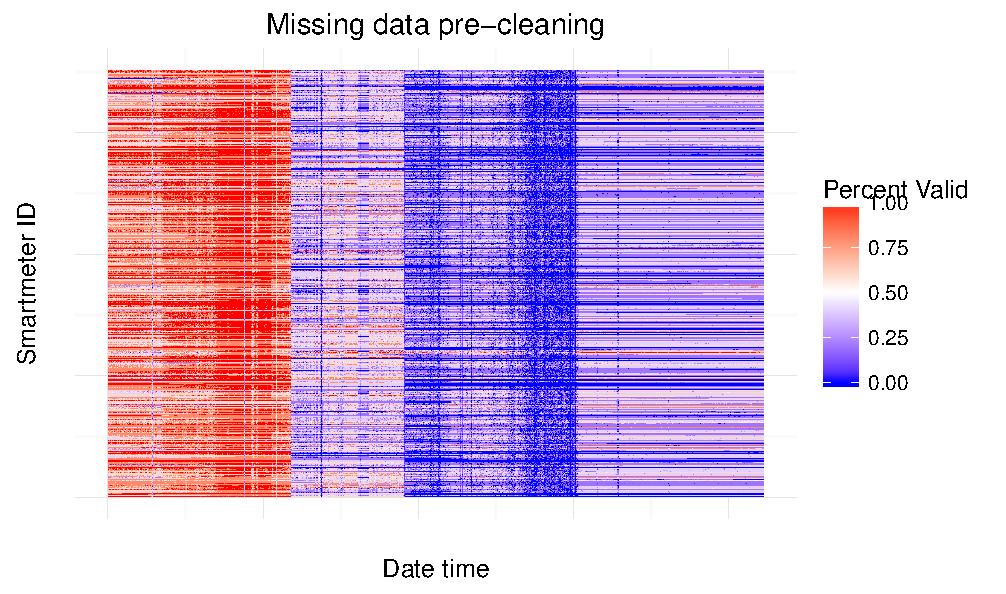
\includegraphics[width=0.49\textwidth]{Figures/unorderedPrecleaningmissing}\label{fig:unordered}
}
\subfloat[missing data with rows and columns ordered by similarity]{
  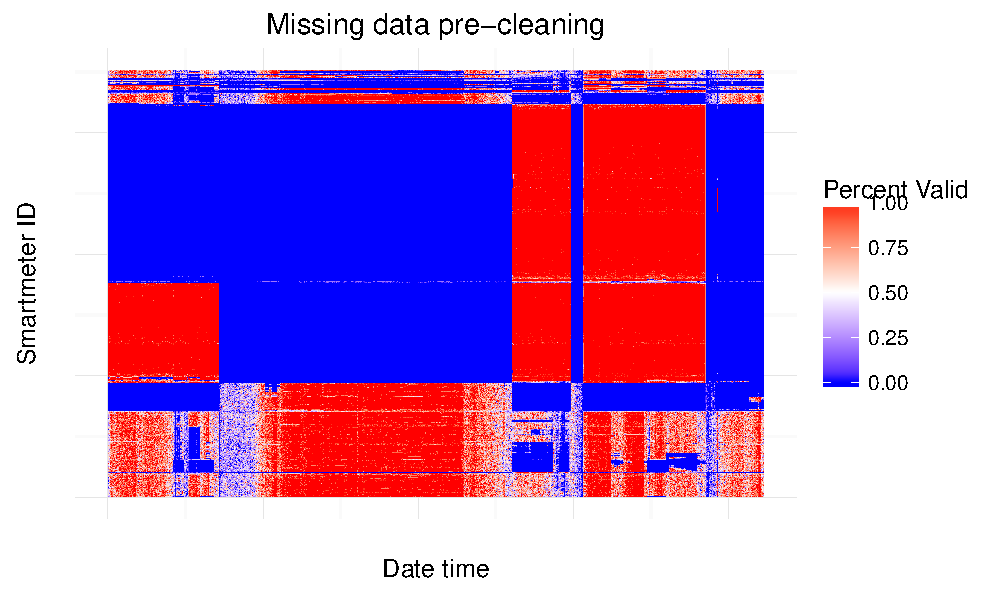
\includegraphics[width=0.49\textwidth]{Figures/Precleaningmissing}\label{fig:ordered}
}

\subfloat[Identifying smart meters that have similar high quality data]{
  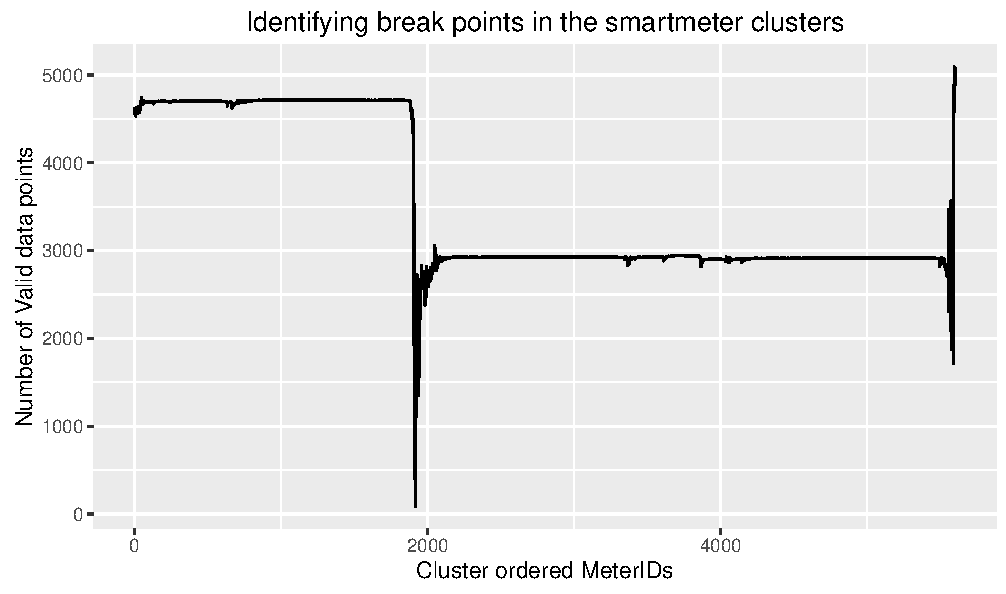
\includegraphics[width=0.49\textwidth]{Figures/breakpoints}\label{fig:breakpoints}
}
\subfloat[Missing data of the selected smart meters in chronological order]{
  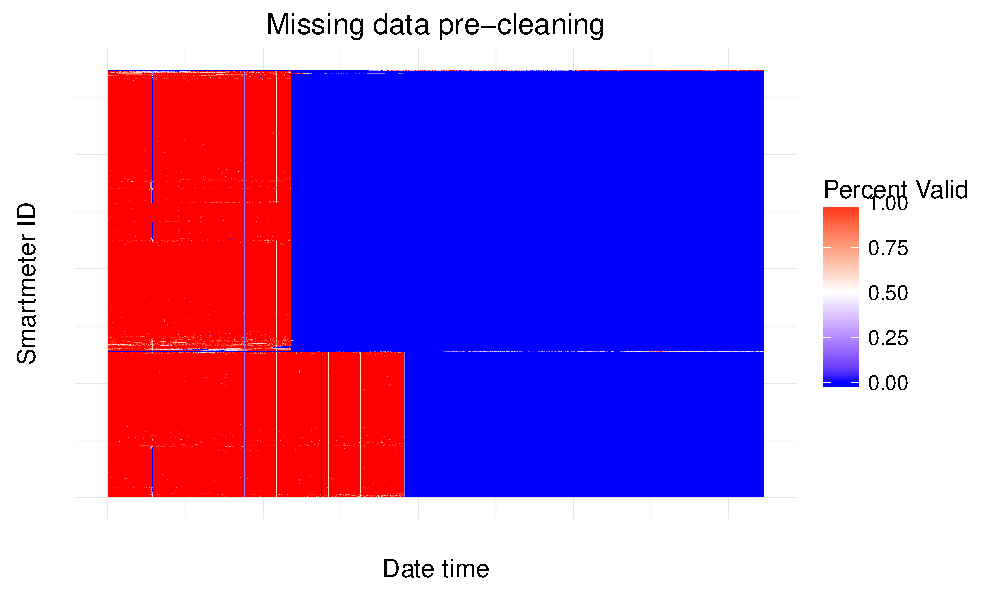
\includegraphics[width=0.49\textwidth]{Figures/LowerPrecleaningmissing}\label{fig:targetordered}
}
\caption[Cleaning the data]{This series of figures shows how the Sub-set of smart meters and time periods were chosen from the raw data.}
\label{fig:dataclean}
\end{figure*}

\begin{figure*}[ht]
\centering
\subfloat[The number of time periods remaining if there is a minimum cut off for valid data]{
  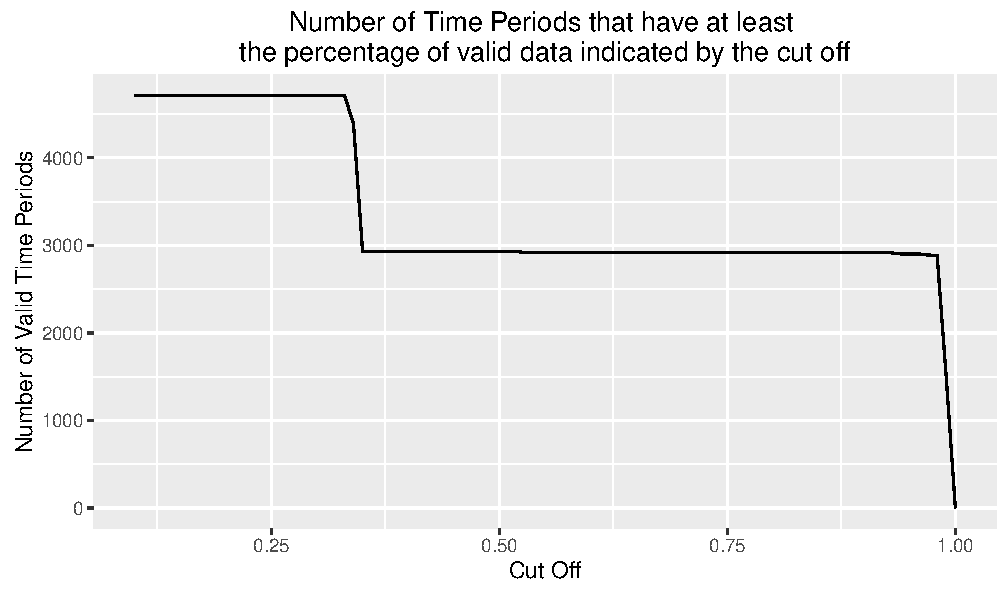
\includegraphics[width=0.49\textwidth]{Figures/NAtimeperiodslowerclust}\label{fig:timecutoff}
}
\subfloat[The figure shows how many smart meters remain if requirements are put on the percentage of time periods that must be valid for the smart meter to be included. As can be seen, the number is much more stable than for the time period figure, however this is mostly due to the time periods have been cleaned first.]{
  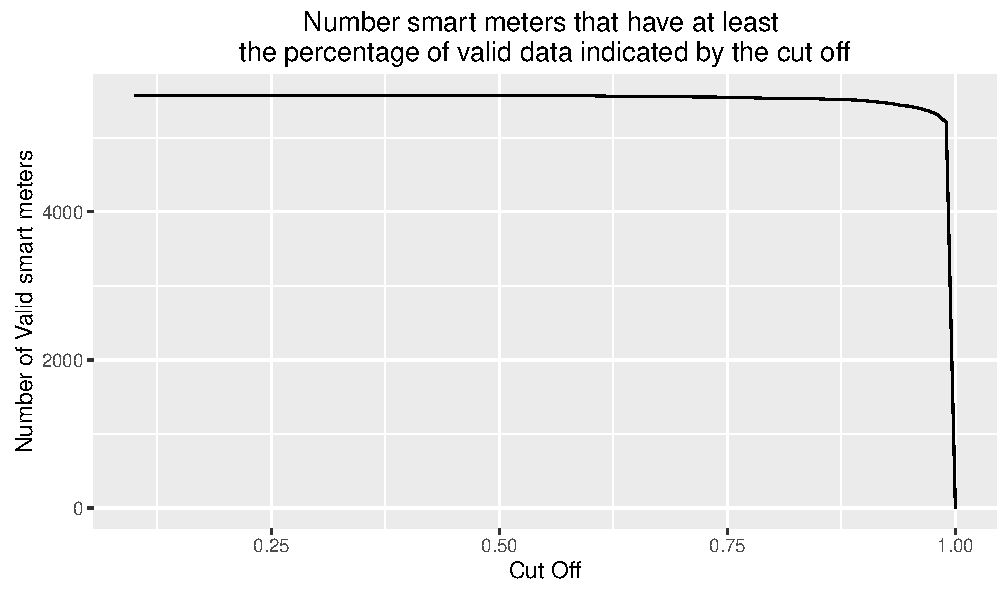
\includegraphics[width=0.49\textwidth]{Figures/NAsmartmeters}\label{fig:metercutoff}
}
%\caption{This series of figures shows how the Sub-set of smart meters and time periods were chosen from the raw data.}
\label{fig:dataclean2}
\end{figure*}


After cleaning there are 242 complete days of 12 half hour periods from 1600 to 2130, there are 239 days that have a comparison day 1 day earlier and 233 days that have a comparison day 1 week earlier and . The total dataset has 14386 NA values.
the dates "2011-06-29", "2011-10-31", "2011-12-12" are missing from the data set due to low valid values further details can be seen in table \ref{tab:nas}. After the  imputation of data described in \ref{sec:imputation}, the 3 missing days were admitted to the data set and  all NA values were filled in.

\begin{table}[ht]
\centering
\begin{tabular}{|l|l|l|l|} \hline
             & Pre Cleaning & Post Cleaning & \% Reduction \\ \hline
Time periods & 10565        & 2915           & 72\%      \\ \hline
Smart Meters & 8790         & 5209          & 41\%      \\ \hline
NA's         & 48\%         & 0\%           & 100\%     \\ \hline
Nodes        & 8798         & 5260          & 40\%      \\ \hline
\end{tabular}
\caption{Summary of the data removal that took place in the cleaning process to reduce the amount of NA's in the dataset.}
\label{tab:nas}
\end{table}

\FloatBarrier

\section{Basic consumption patterns}
\label{sec:basicconsum}
A brief visual analysis of the data shows a few key insights. Figure \ref{fig:PortfolioLoad} breaks out the the load profile per week day, it shows that independent of day of the week all evening peaks look roughly the same. However the weekend peak is slightly before the week days, peaking about an hour earlier, in addition Saturday has the lowest average consumption. Aggregating the consumption to total kWh per day and comparing daily consumption across months, a clear pattern emerges as shown in figure \ref{fig:DailyConsumption}. As the days get darker and colder energy consumption increases, this is intuitive as people are more likely to spend time indoors, have the lights on, and use heating. 

As this project relies on finding correlations between smart meters, it is interesting to look at how much correlation there is within smart meters. This means looking at a single smart meter's correlation with itself across multiple days. Figure \ref{fig:MeanAbsCorr} shows a density distribution of the absolute correlation across 50 randomly sampled smart meters. If people led very regimented lives and did exactly the same thing every day then the average score would be 1, conversely no pattern would get a score of 0. The distribution shows a mean score of 0.3 which is quite low, suggesting that there is not strong structure among individual energy consumption. The unexpectedly low levels of correlation may be due to the low absolute levels of electricity consumption relative to the total energy consumption for the household, see Appendix \ref{sec:Energybreakdown} for more details and discussion. 


\begin{figure}
    \centering
    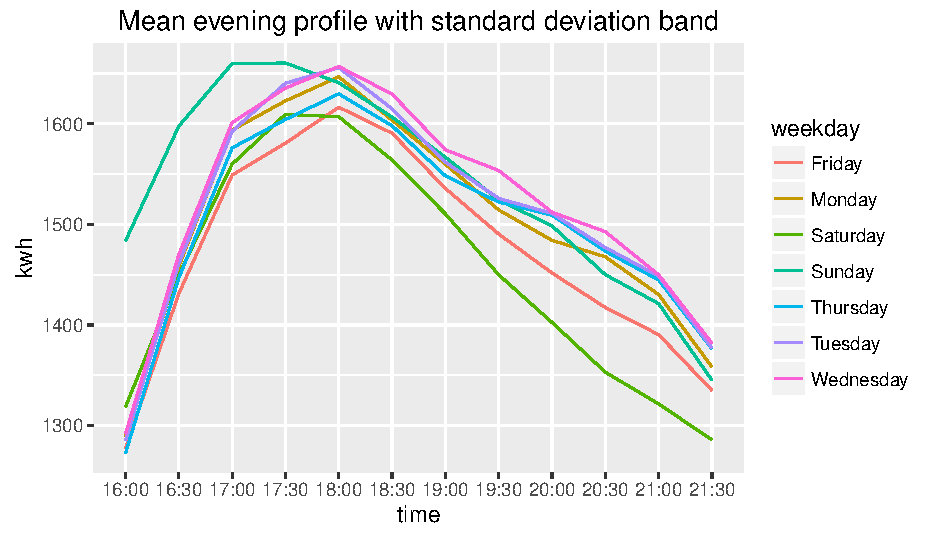
\includegraphics[width = \textwidth]{Figures/Results/PortfolioLoad}
    \caption[Portfolio load by day]{The figure shows the portfolio load across all weekdays, as can be seen the load on the system peaks at about 1800 across all weekdays. The weekend peak is slightly earlier, peaking about an hour earlier, in addition Saturday has the lowest average consumption.}
    \label{fig:PortfolioLoad}
\end{figure}

\begin{figure}
    \centering
    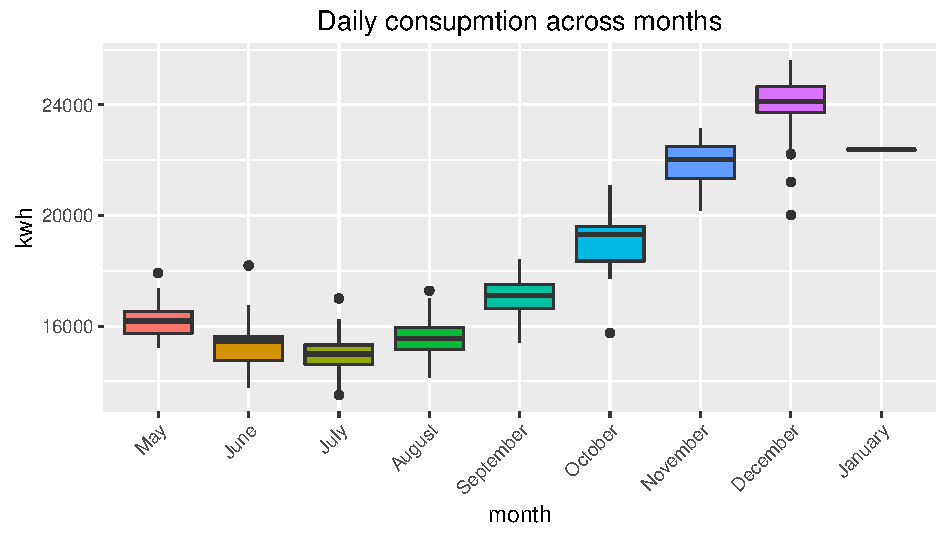
\includegraphics[width = \textwidth]{Figures/Results/DailyConsumptionMonths}
    \caption[Daily consumption across months]{As can be seen the consumption of electricity increases as the days get darker and colder, requiring more energy in the form of heat an light.}
    \label{fig:DailyConsumption}
\end{figure}

\begin{figure}
    \centering
    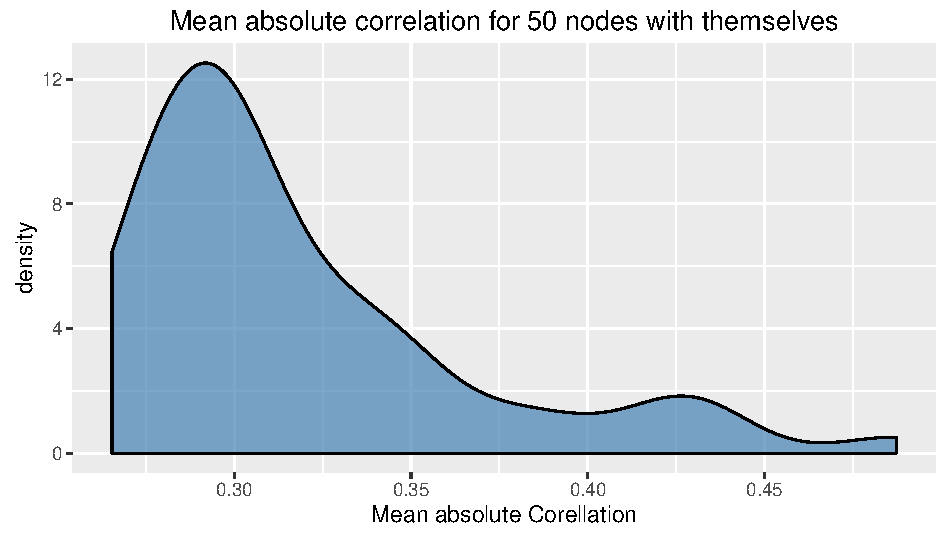
\includegraphics[width = \textwidth]{Figures/Results/MeanAbsCorr}
    \caption[Node Mean absolute correlation]{This figure was made by Taking a node and find it's mean absolute correlation with itself across all days, and repeating with 50 randomly selected nodes. The resulting vector of scores are then made into a density plot. the right skew shows that the majority of nodes have very low self-correlation suggesting that there is little fixed pattern to behaviour.}
    \label{fig:MeanAbsCorr}
\end{figure}

\section{Summary}

This chapter explains the method and results of the cleaning process for the TC1a dataset. The dataset had 48\% missing values during the evening peak period this was reduced to slightly over 0\% and the remaining missing values were imputed using node/day/time mean. Cleaning used a combination of hierarchical clustering,visualisation and minimum data quality decisions in order to produce the final dataset.


